
\renewcommand{\hbAppendixPrefix}{D}

\renewcommand{\thefigure}{\hbAppendixPrefix\arabic{figure}}
\setcounter{figure}{0}
\renewcommand{\thetable}{\hbAppendixPrefix\arabic{table}}
\setcounter{table}{0}
\renewcommand{\theequation}{\hbAppendixPrefix\arabic{equation}}
\setcounter{equation}{0}

\section{Supplementary Material 1 for Chapter \ref{ch:hpc}} \label{apx:sm1-hpc}

\begin{figure}[H]
    \caption{Solution improvement process.}
    \centering
    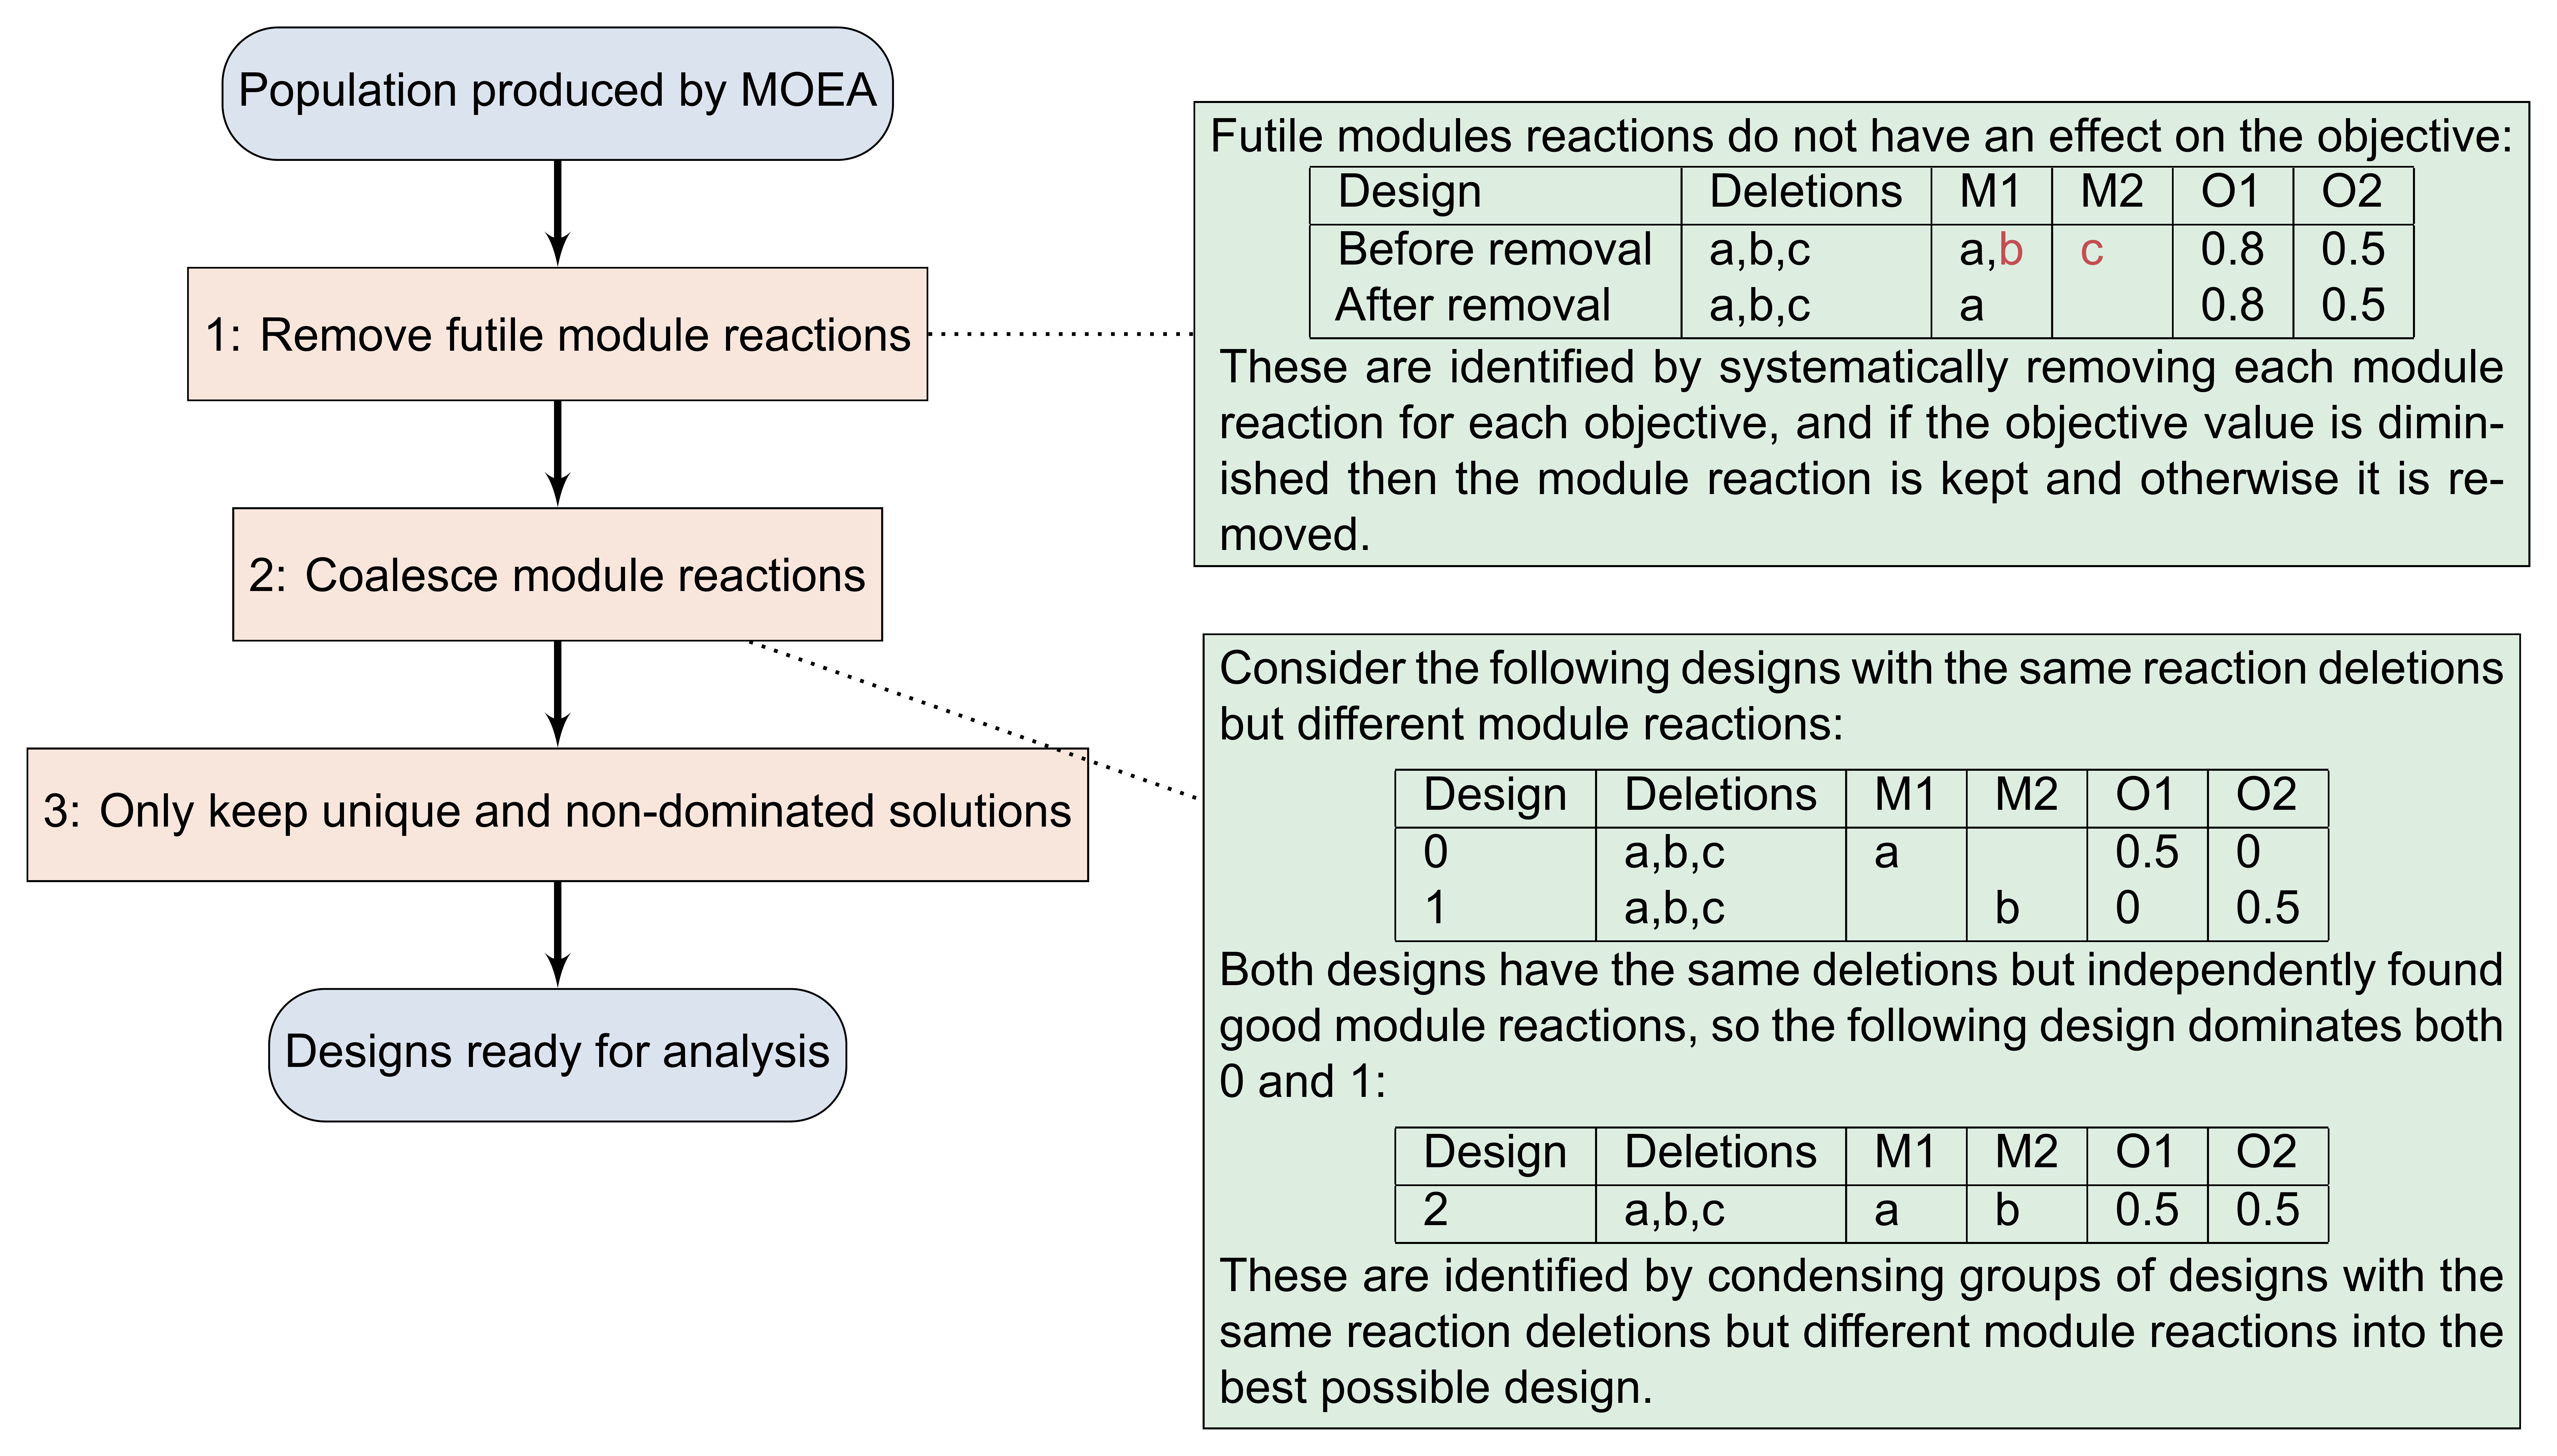
\includegraphics[width=\textwidth,keepaspectratio]{processing.png}
    \label{fig7:processing}
\end{figure}

\begin{figure}[H]
    \caption[Chemical properties of the product library]{Chemical properties of the product library. DoR is the degree of reduction (mol e\textsuperscript{-}/ mol C), which is computed assuming a constant valency of 4,1,-2, and 5 for C,H,O, and P, respectively.  For reference, ethanol has 2 carbon atoms, a molecular weight of 46 g/mol, and a DoR of 6 (mol e\textsuperscript{-}/mol C). The molecular weight and the number of carbon atoms have a Pearson correlation coefficient (pcc) of 0.98, while DoR and the molecular weight only have a pcc of 0.42.}
    \centering
    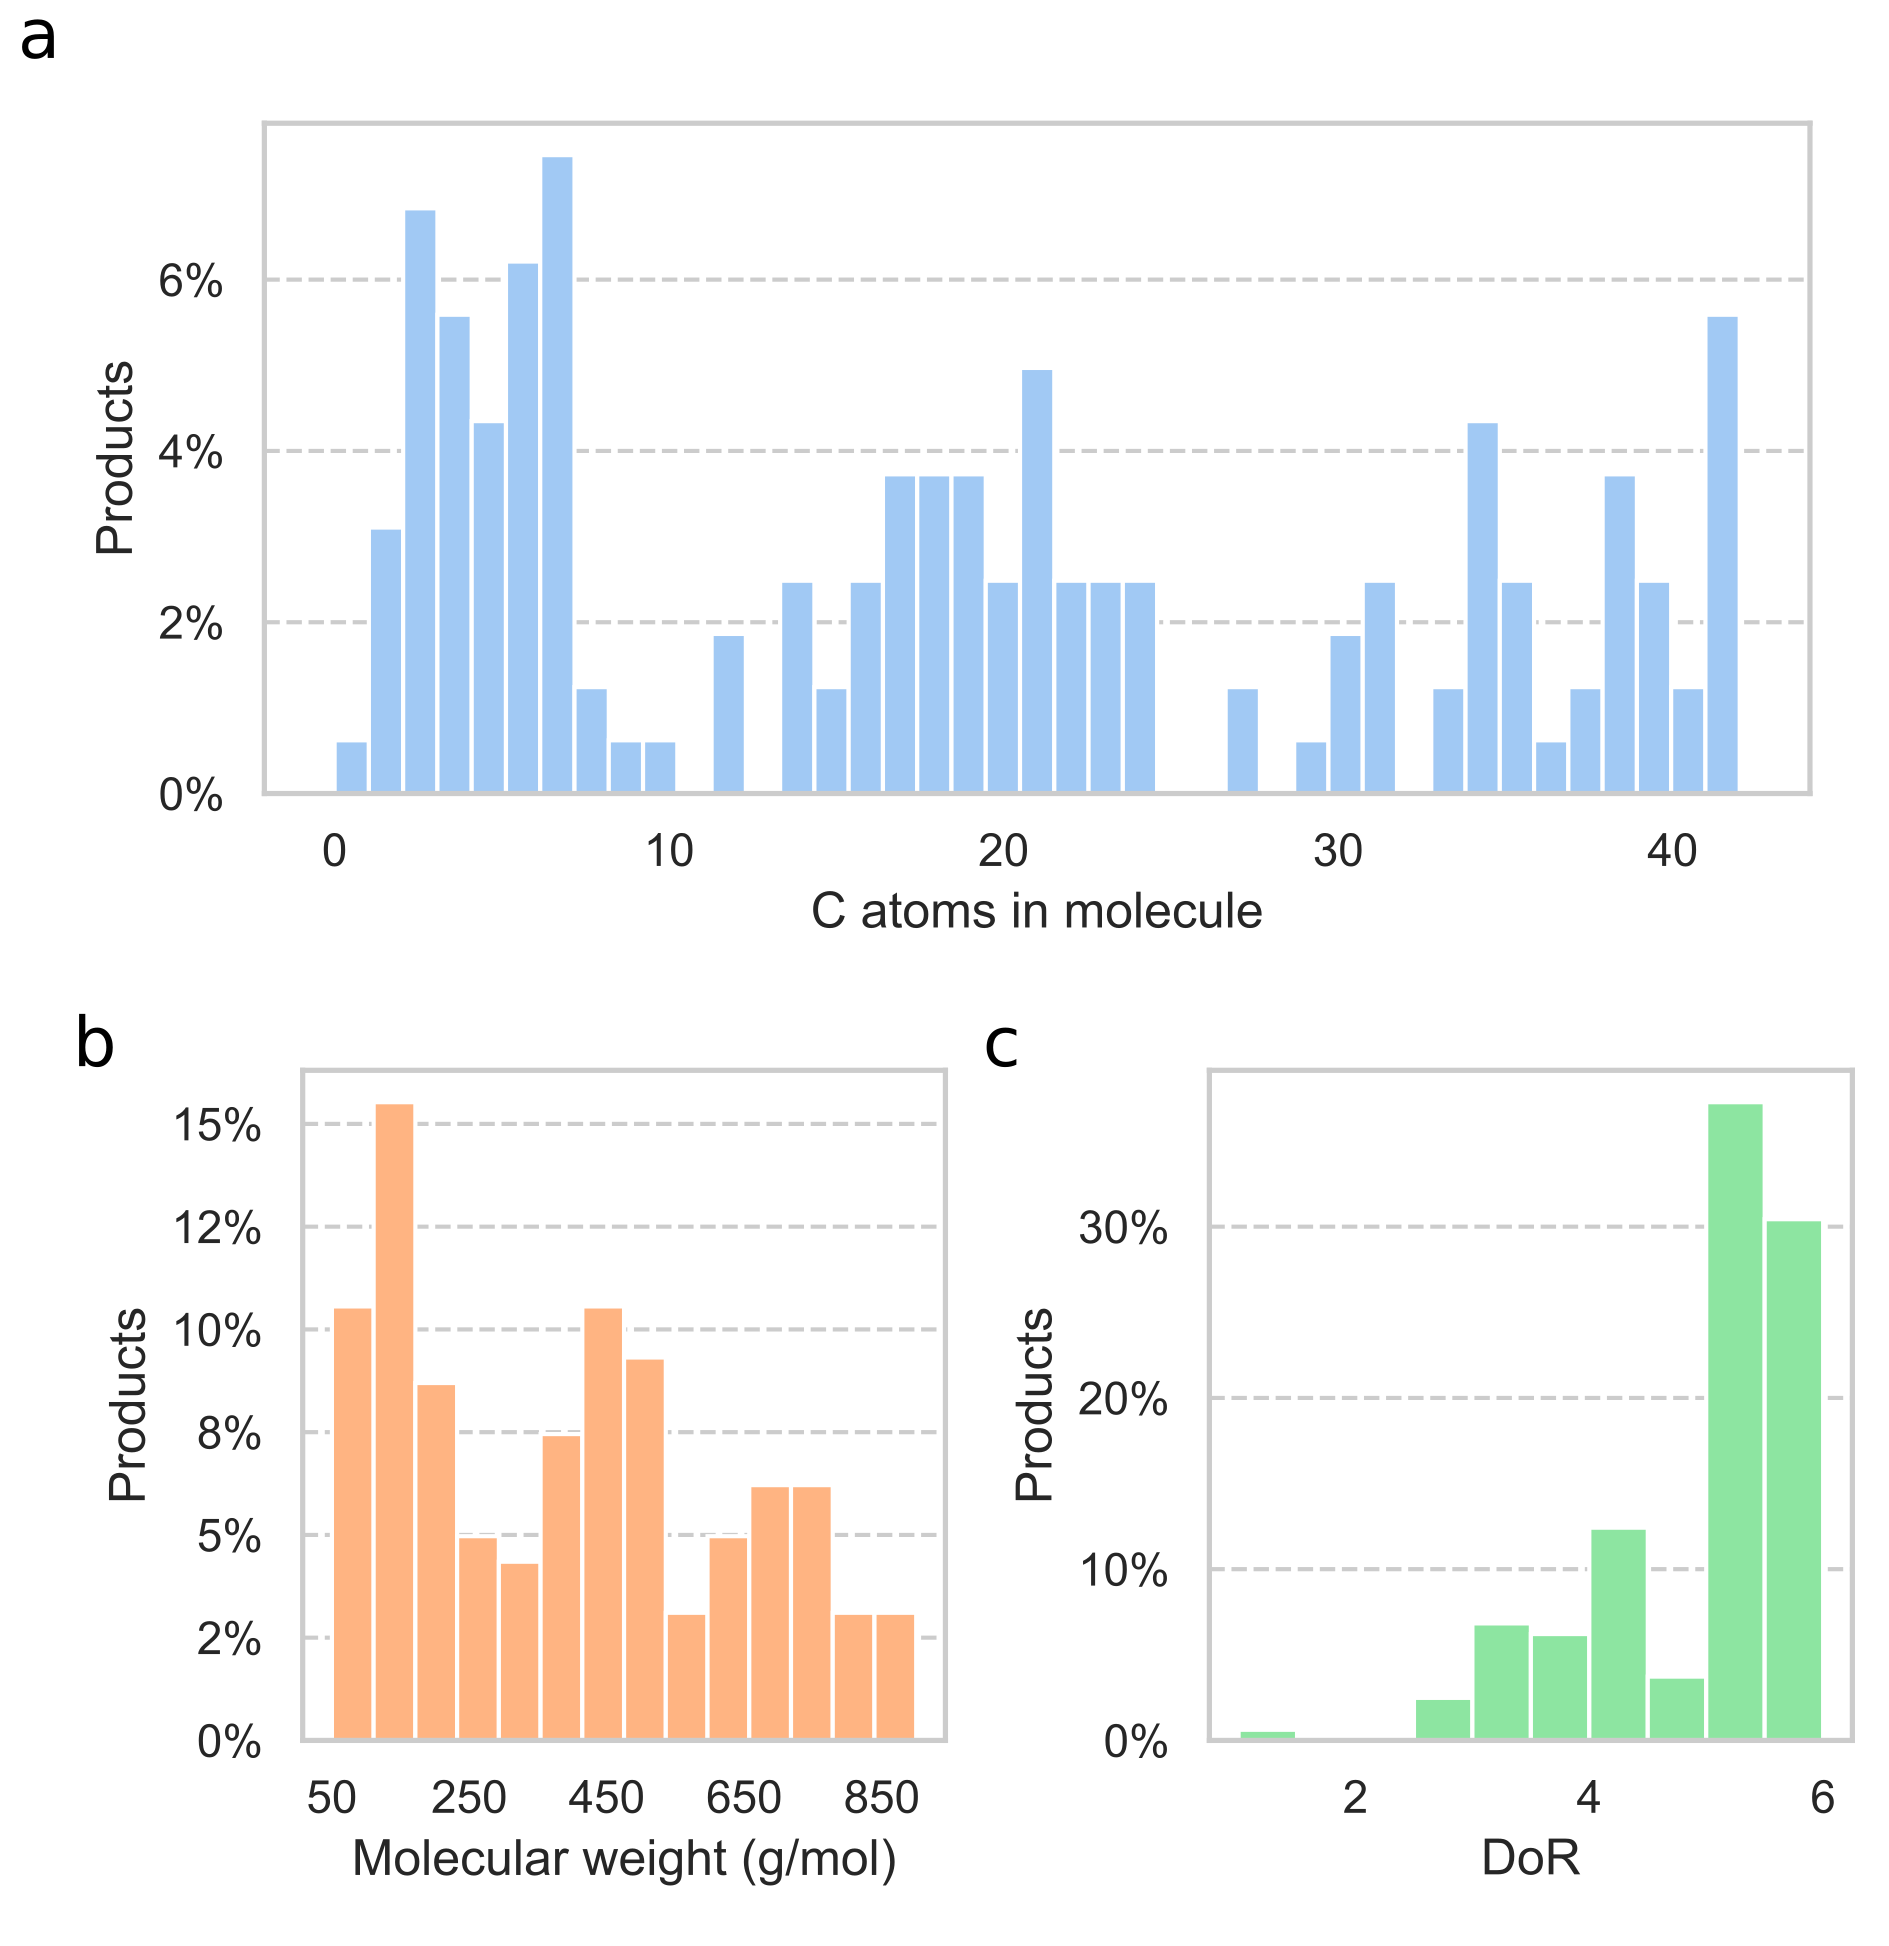
\includegraphics[width=.8\textwidth,keepaspectratio]{biochemical-native.png}
    \label{fig7:biochemical-properties}
\end{figure}

\begin{figure}[H]
    \caption[ModCell-HPC benchmarking with 20 products]{ModCell-HPC benchmarking with 20 products and design parameters $\alpha=6, \,\beta=1$. For a given run time, this analysis scans through all the combinations of migration interval, migration policy, and population size. Note that coverage values are not directly comparable between run times since the use a different reference Pareto front.}
    \centering
    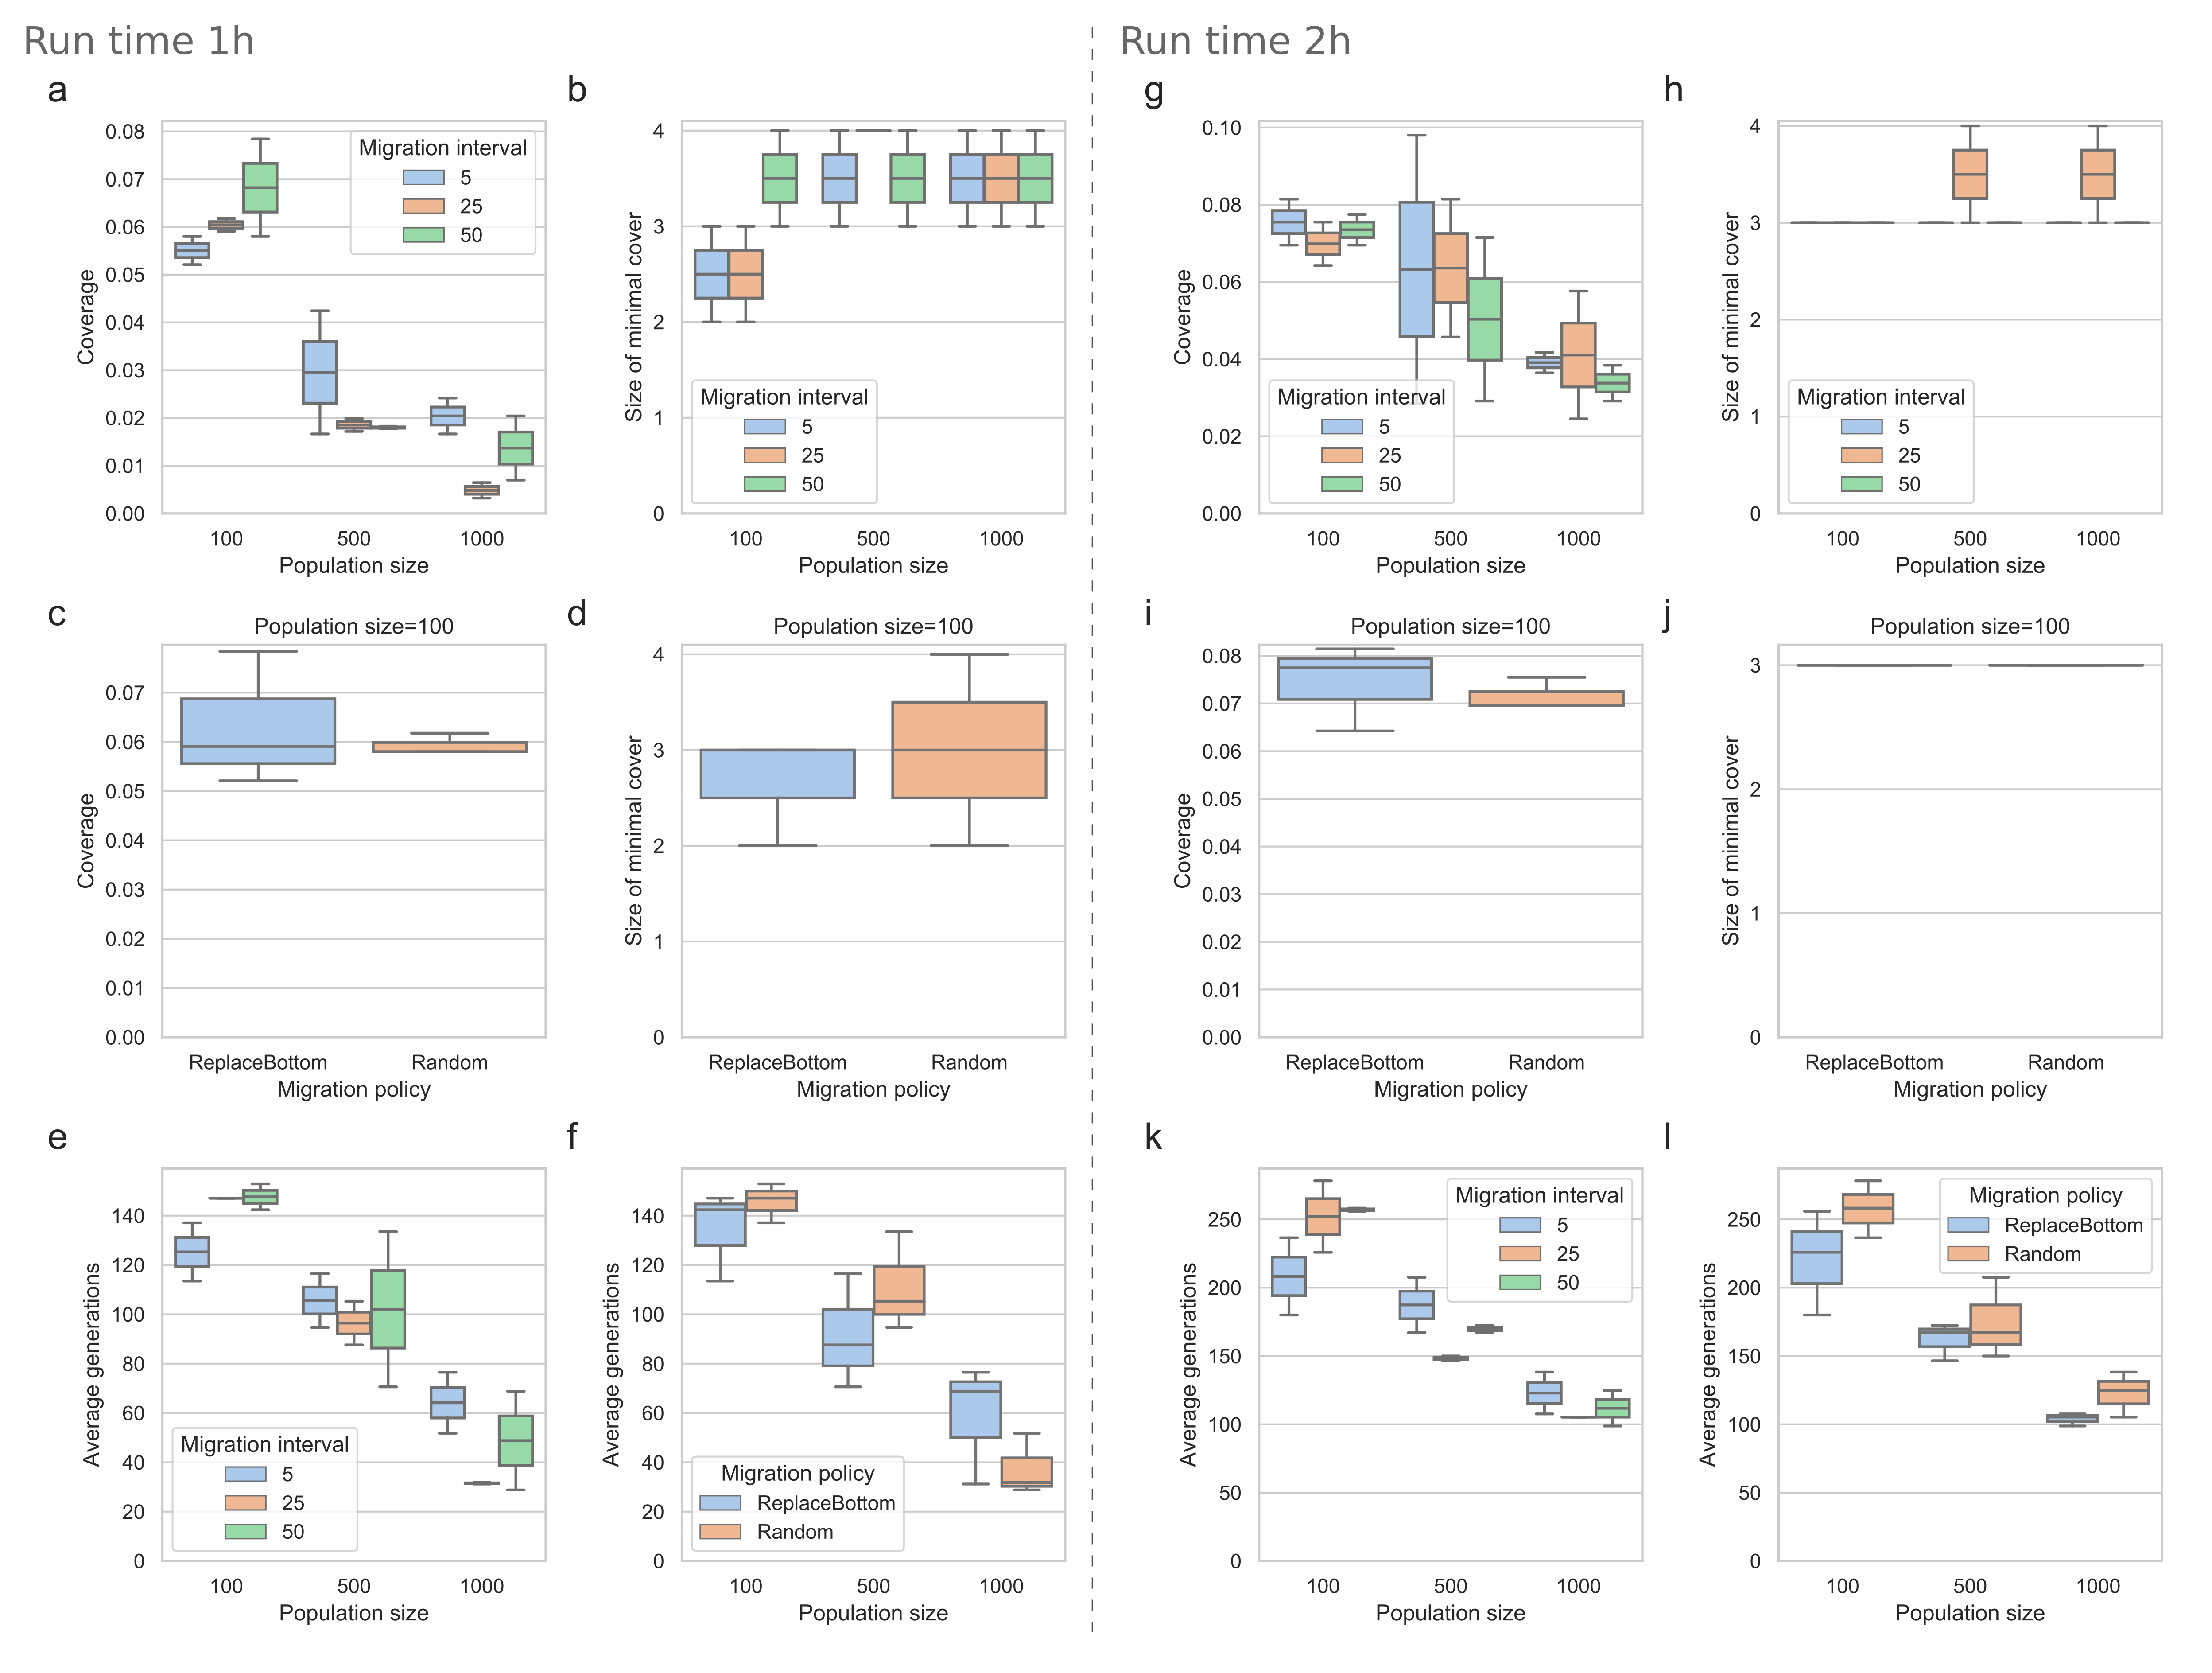
\includegraphics[width=\textwidth,keepaspectratio]{benchmark-gem-model.png}
    \label{fig7:benchmark-20prod}
\end{figure}

\begin{figure}[H]
    \caption[Compatibility distributions]{Compatibility of all designs in a Pareto front as a result of the design parameters. Each panel corresponds to a unique carbon source as the only difference in model configuration.}
    \centering
    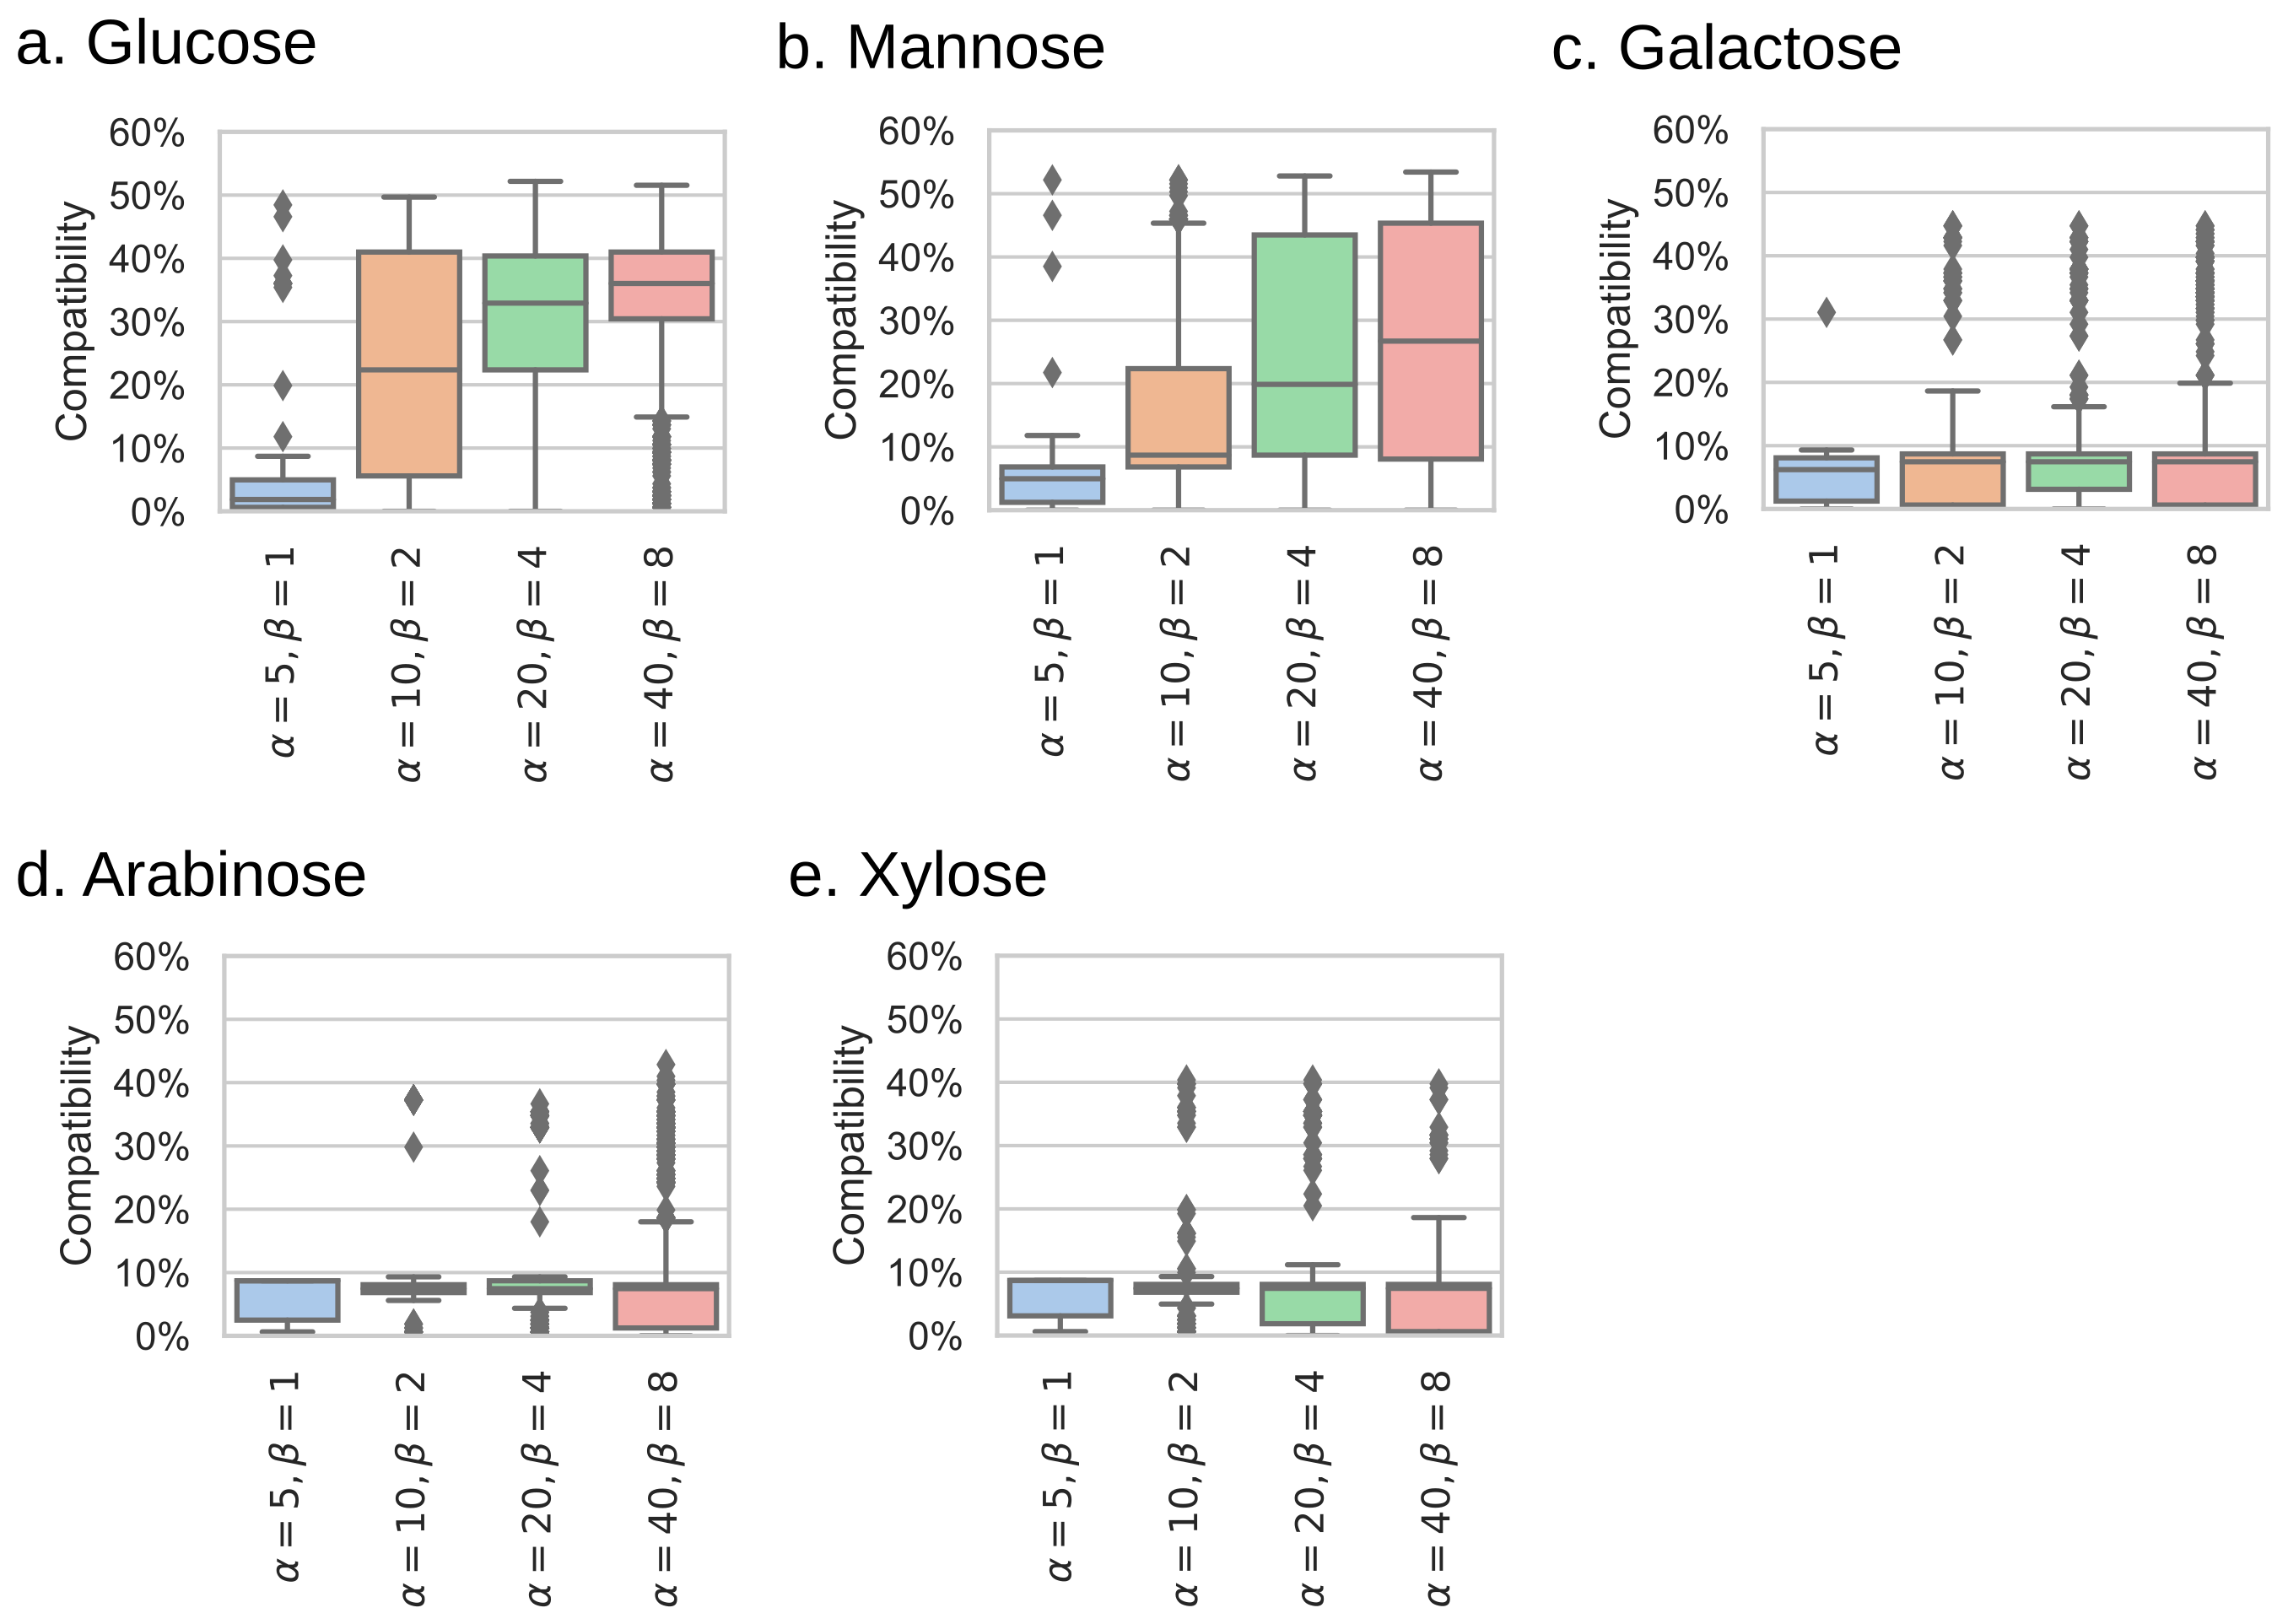
\includegraphics[width=\textwidth,keepaspectratio]{sugars-compatibility.png}
    \label{fig7:parameter-scan}
\end{figure}

\begin{figure}[H]
    \caption[Bipartite graph of minimal covers]{Bipartite graph representing minimal covers for design parameters $\alpha=5$ and $\beta=1$. Covers are colored in red and labeled with letters, while designs are colored in blue.
        %Some designs appear in more covers (e.g., 121).
        All minimal covers are:
            a: [101, 109, 121],
            b: [109, 121, 124],
            c: [101, 110, 121],
            d: [25, 101, 121],
            e: [82, 101, 121],
            f: [110, 121, 124],
            g: [97, 109, 121],
            h: [97, 110, 121],
            i: [25, 97, 121],
            j: [25, 121, 124],
            k: [82, 121, 124],
            l: [82, 97, 121].
            }
    \centering
    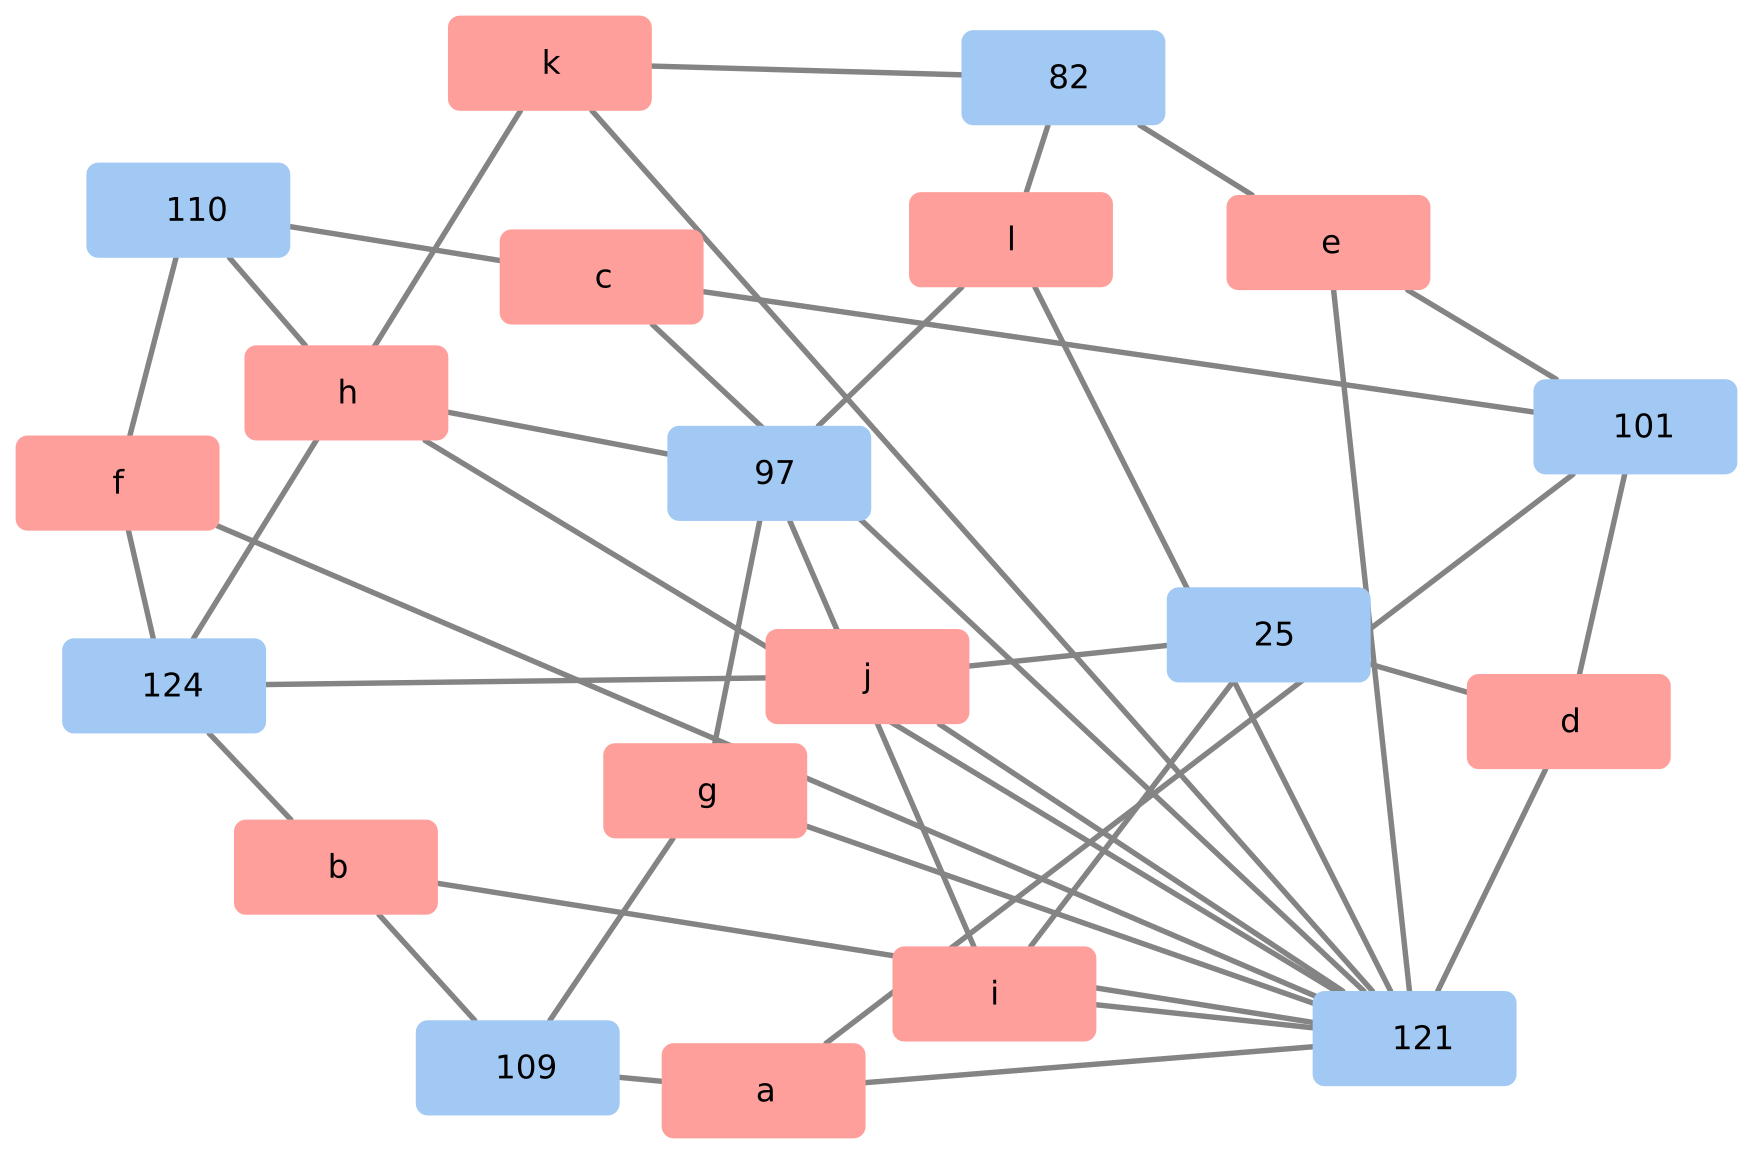
\includegraphics[width=\textwidth,keepaspectratio]{cover-graph.png}
    \label{fig7:cover-graph}
\end{figure}
